%!TEX TS-program = xelatex
\documentclass[11pt]{article}

\usepackage[english]{babel}

\usepackage{amsmath,amssymb,amsfonts}
\usepackage[utf8]{inputenc}
\usepackage[T1]{fontenc}
\usepackage{stix2}
\usepackage[scaled]{helvet}
\usepackage[scaled]{inconsolata}

\usepackage{lastpage}

\usepackage{setspace}

\usepackage{ccicons}

\usepackage[hang,flushmargin]{footmisc}

\usepackage{geometry}

\setlength{\parindent}{0pt}
\setlength{\parskip}{6pt plus 2pt minus 1pt}

\usepackage{fancyhdr}
\renewcommand{\headrulewidth}{0pt}\providecommand{\tightlist}{%
  \setlength{\itemsep}{0pt}\setlength{\parskip}{0pt}}

\makeatletter
\newcounter{tableno}
\newenvironment{tablenos:no-prefix-table-caption}{
  \caption@ifcompatibility{}{
    \let\oldthetable\thetable
    \let\oldtheHtable\theHtable
    \renewcommand{\thetable}{tableno:\thetableno}
    \renewcommand{\theHtable}{tableno:\thetableno}
    \stepcounter{tableno}
    \captionsetup{labelformat=empty}
  }
}{
  \caption@ifcompatibility{}{
    \captionsetup{labelformat=default}
    \let\thetable\oldthetable
    \let\theHtable\oldtheHtable
    \addtocounter{table}{-1}
  }
}
\makeatother

\usepackage{array}
\newcommand{\PreserveBackslash}[1]{\let\temp=\\#1\let\\=\temp}
\let\PBS=\PreserveBackslash

\usepackage[breaklinks=true]{hyperref}
\hypersetup{colorlinks,%
citecolor=blue,%
filecolor=blue,%
linkcolor=blue,%
urlcolor=blue}
\usepackage{url}

\usepackage{caption}
\setcounter{secnumdepth}{0}
\usepackage{cleveref}

\usepackage{graphicx}
\makeatletter
\def\maxwidth{\ifdim\Gin@nat@width>\linewidth\linewidth
\else\Gin@nat@width\fi}
\makeatother
\let\Oldincludegraphics\includegraphics
\renewcommand{\includegraphics}[1]{\Oldincludegraphics[width=\maxwidth]{#1}}

\usepackage{longtable}
\usepackage{booktabs}

\usepackage{color}
\usepackage{fancyvrb}
\newcommand{\VerbBar}{|}
\newcommand{\VERB}{\Verb[commandchars=\\\{\}]}
\DefineVerbatimEnvironment{Highlighting}{Verbatim}{commandchars=\\\{\}}
% Add ',fontsize=\small' for more characters per line
\usepackage{framed}
\definecolor{shadecolor}{RGB}{248,248,248}
\newenvironment{Shaded}{\begin{snugshade}}{\end{snugshade}}
\newcommand{\KeywordTok}[1]{\textcolor[rgb]{0.13,0.29,0.53}{\textbf{#1}}}
\newcommand{\DataTypeTok}[1]{\textcolor[rgb]{0.13,0.29,0.53}{#1}}
\newcommand{\DecValTok}[1]{\textcolor[rgb]{0.00,0.00,0.81}{#1}}
\newcommand{\BaseNTok}[1]{\textcolor[rgb]{0.00,0.00,0.81}{#1}}
\newcommand{\FloatTok}[1]{\textcolor[rgb]{0.00,0.00,0.81}{#1}}
\newcommand{\ConstantTok}[1]{\textcolor[rgb]{0.00,0.00,0.00}{#1}}
\newcommand{\CharTok}[1]{\textcolor[rgb]{0.31,0.60,0.02}{#1}}
\newcommand{\SpecialCharTok}[1]{\textcolor[rgb]{0.00,0.00,0.00}{#1}}
\newcommand{\StringTok}[1]{\textcolor[rgb]{0.31,0.60,0.02}{#1}}
\newcommand{\VerbatimStringTok}[1]{\textcolor[rgb]{0.31,0.60,0.02}{#1}}
\newcommand{\SpecialStringTok}[1]{\textcolor[rgb]{0.31,0.60,0.02}{#1}}
\newcommand{\ImportTok}[1]{#1}
\newcommand{\CommentTok}[1]{\textcolor[rgb]{0.56,0.35,0.01}{\textit{#1}}}
\newcommand{\DocumentationTok}[1]{\textcolor[rgb]{0.56,0.35,0.01}{\textbf{\textit{#1}}}}
\newcommand{\AnnotationTok}[1]{\textcolor[rgb]{0.56,0.35,0.01}{\textbf{\textit{#1}}}}
\newcommand{\CommentVarTok}[1]{\textcolor[rgb]{0.56,0.35,0.01}{\textbf{\textit{#1}}}}
\newcommand{\OtherTok}[1]{\textcolor[rgb]{0.56,0.35,0.01}{#1}}
\newcommand{\FunctionTok}[1]{\textcolor[rgb]{0.00,0.00,0.00}{#1}}
\newcommand{\VariableTok}[1]{\textcolor[rgb]{0.00,0.00,0.00}{#1}}
\newcommand{\ControlFlowTok}[1]{\textcolor[rgb]{0.13,0.29,0.53}{\textbf{#1}}}
\newcommand{\OperatorTok}[1]{\textcolor[rgb]{0.81,0.36,0.00}{\textbf{#1}}}
\newcommand{\BuiltInTok}[1]{#1}
\newcommand{\ExtensionTok}[1]{#1}
\newcommand{\PreprocessorTok}[1]{\textcolor[rgb]{0.56,0.35,0.01}{\textit{#1}}}
\newcommand{\AttributeTok}[1]{\textcolor[rgb]{0.77,0.63,0.00}{#1}}
\newcommand{\RegionMarkerTok}[1]{#1}
\newcommand{\InformationTok}[1]{\textcolor[rgb]{0.56,0.35,0.01}{\textbf{\textit{#1}}}}
\newcommand{\WarningTok}[1]{\textcolor[rgb]{0.56,0.35,0.01}{\textbf{\textit{#1}}}}
\newcommand{\AlertTok}[1]{\textcolor[rgb]{0.94,0.16,0.16}{#1}}
\newcommand{\ErrorTok}[1]{\textcolor[rgb]{0.64,0.00,0.00}{\textbf{#1}}}
\newcommand{\NormalTok}[1]{#1}

\newlength{\cslhangindent}
\setlength{\cslhangindent}{1.5em}
\newlength{\csllabelwidth}
\setlength{\csllabelwidth}{3em}
\newenvironment{CSLReferences}[3] % #1 hanging-ident, #2 entry spacing
 {% don't indent paragraphs
  \setlength{\parindent}{0pt}
  % turn on hanging indent if param 1 is 1
  \ifodd #1 \everypar{\setlength{\hangindent}{\cslhangindent}}\ignorespaces\fi
  % set entry spacing
  \ifnum #2 > 0
  \setlength{\parskip}{#2\baselineskip}
  \fi
 }%
 {}
\usepackage{calc} % for \widthof, \maxof
\newcommand{\CSLBlock}[1]{#1\hfill\break}
\newcommand{\CSLLeftMargin}[1]{\parbox[t]{\maxof{\widthof{#1}}{\csllabelwidth}}{#1}}
\newcommand{\CSLRightInline}[1]{\parbox[t]{\linewidth}{#1}}
\newcommand{\CSLIndent}[1]{\hspace{\cslhangindent}#1}\geometry{verbose,letterpaper,tmargin=2.2cm,bmargin=2.2cm,lmargin=2.2cm,rmargin=2.2cm}

\usepackage{lineno}
\usepackage[nolists,noheads]{endfloat}

\pagestyle{plain}

\tolerance=1
\emergencystretch=\maxdimen
\hyphenpenalty=10000
\hbadness=10000

\doublespacing

\fancypagestyle{normal}
{
  \fancyhf{}
  \fancyfoot[R]{\footnotesize\sffamily\thepage\ of \pageref*{LastPage}}
}
\begin{document}
\raggedright
\thispagestyle{empty}
{\Large\bfseries\sffamily NeutralLandscapes.jl: a library for efficient
generation of neutral landscapes with temporal change}
\vskip 5em

%
\href{https://orcid.org/0000-0002-6506-6487}{Michael D.\,Catchen}%
%
\,\textsuperscript{1,2}

\textsuperscript{1}\,McGill University\quad \textsuperscript{2}\,Québec
Centre for Biodiversity Sciences


\textbf{Correspondance to:}\\
Michael D. Catchen --- \texttt{michael.catchen@mail.mcgill.ca}\\

\vfill
This work is released by its authors under a CC-BY 4.0 license\hfill\ccby\\
Last revision: \emph{\today}

\clearpage
\thispagestyle{empty}

\vfill
Soon to be a paper, maybe. TK authors, MKB,VB,RS,TP



\vfill

\clearpage
\linenumbers
\pagestyle{normal}

\hypertarget{introduction}{%
\section{Introduction}\label{introduction}}

Neutral landscapes are increasingly used in ecological and evolutionary
studies to provide a null expectation of the variance of a given metric
over space.

Wide range of disciplines: from landscape genetics {[}{]}, to spatial
ecology {[}{]}, and biogeography {[}{]}.

As biodiversity science becomes increasingly concerned with temporal
change and its consequences, its clear there is a gap generating neutral
landscapes that change over time. In this ms we present how
\texttt{NeutralLandscapes.jl} is orders of magnitudes faster than
packages \texttt{nlmpy} (in python) or \texttt{NLMR} (in R). In addition
we then present a novel method for generating landscape change with
prescribed levels of spatial and temporal autocorrelation.

\hypertarget{software-overview}{%
\section{Software Overview}\label{software-overview}}

This software can generate neutral landscapes using several methods,
enables masking and works with other julia packages.

fig.~\ref{fig:allmethods} shows a replica of Figure 1 from
(\textbf{nlmpycite?}), which shows the capacity of the library to
generate different types of neutral landscapes, and then apply masks and
categorical classifcation to them.

Table of methods.

\begin{longtable}[]{@{}llllll@{}}
\toprule
\begin{minipage}[b]{0.35\columnwidth}\raggedright
Model\strut
\end{minipage} & \begin{minipage}[b]{0.07\columnwidth}\raggedright
nlmpy?\strut
\end{minipage} & \begin{minipage}[b]{0.05\columnwidth}\raggedright
NLMR\strut
\end{minipage} & \begin{minipage}[b]{0.33\columnwidth}\raggedright
Description\strut
\end{minipage} & \begin{minipage}[b]{0.02\columnwidth}\raggedright
Reference\strut
\end{minipage} & \begin{minipage}[b]{0.02\columnwidth}\raggedright
Aliases\strut
\end{minipage}\tabularnewline
\midrule
\endhead
\begin{minipage}[t]{0.35\columnwidth}\raggedright
No gradient\strut
\end{minipage} & \begin{minipage}[t]{0.07\columnwidth}\raggedright
x\strut
\end{minipage} & \begin{minipage}[t]{0.05\columnwidth}\raggedright
x\strut
\end{minipage} & \begin{minipage}[t]{0.33\columnwidth}\raggedright
Each cell is drawn randomly\strut
\end{minipage} & \begin{minipage}[t]{0.02\columnwidth}\raggedright
\strut
\end{minipage} & \begin{minipage}[t]{0.02\columnwidth}\raggedright
\strut
\end{minipage}\tabularnewline
\begin{minipage}[t]{0.35\columnwidth}\raggedright
Planar gradient\strut
\end{minipage} & \begin{minipage}[t]{0.07\columnwidth}\raggedright
x\strut
\end{minipage} & \begin{minipage}[t]{0.05\columnwidth}\raggedright
x\strut
\end{minipage} & \begin{minipage}[t]{0.33\columnwidth}\raggedright
A gradient from low to high at a given angle\strut
\end{minipage} & \begin{minipage}[t]{0.02\columnwidth}\raggedright
\strut
\end{minipage} & \begin{minipage}[t]{0.02\columnwidth}\raggedright
\strut
\end{minipage}\tabularnewline
\begin{minipage}[t]{0.35\columnwidth}\raggedright
Distance gradient\strut
\end{minipage} & \begin{minipage}[t]{0.07\columnwidth}\raggedright
x\strut
\end{minipage} & \begin{minipage}[t]{0.05\columnwidth}\raggedright
x\strut
\end{minipage} & \begin{minipage}[t]{0.33\columnwidth}\raggedright
Each cell is the distance between that cell and a location\strut
\end{minipage} & \begin{minipage}[t]{0.02\columnwidth}\raggedright
\strut
\end{minipage} & \begin{minipage}[t]{0.02\columnwidth}\raggedright
\strut
\end{minipage}\tabularnewline
\begin{minipage}[t]{0.35\columnwidth}\raggedright
Random rectuangular cluster\strut
\end{minipage} & \begin{minipage}[t]{0.07\columnwidth}\raggedright
x\strut
\end{minipage} & \begin{minipage}[t]{0.05\columnwidth}\raggedright
x\strut
\end{minipage} & \begin{minipage}[t]{0.33\columnwidth}\raggedright
Covers the plane in random rectanges until covered\strut
\end{minipage} & \begin{minipage}[t]{0.02\columnwidth}\raggedright
\strut
\end{minipage} & \begin{minipage}[t]{0.02\columnwidth}\raggedright
\strut
\end{minipage}\tabularnewline
\begin{minipage}[t]{0.35\columnwidth}\raggedright
Random element nearest-neighbor\strut
\end{minipage} & \begin{minipage}[t]{0.07\columnwidth}\raggedright
x\strut
\end{minipage} & \begin{minipage}[t]{0.05\columnwidth}\raggedright
x*\strut
\end{minipage} & \begin{minipage}[t]{0.33\columnwidth}\raggedright
Discrete categories based on distance a set of \texttt{n} random
points\strut
\end{minipage} & \begin{minipage}[t]{0.02\columnwidth}\raggedright
\strut
\end{minipage} & \begin{minipage}[t]{0.02\columnwidth}\raggedright
\texttt{nlm\_mosaictess}, k-means\strut
\end{minipage}\tabularnewline
\begin{minipage}[t]{0.35\columnwidth}\raggedright
Random cluster nearest-neighbor\strut
\end{minipage} & \begin{minipage}[t]{0.07\columnwidth}\raggedright
x\strut
\end{minipage} & \begin{minipage}[t]{0.05\columnwidth}\raggedright
x\strut
\end{minipage} & \begin{minipage}[t]{0.33\columnwidth}\raggedright
Starts with \(n\) seed points and grows clusters probabilistically\strut
\end{minipage} & \begin{minipage}[t]{0.02\columnwidth}\raggedright
\strut
\end{minipage} & \begin{minipage}[t]{0.02\columnwidth}\raggedright
\strut
\end{minipage}\tabularnewline
\begin{minipage}[t]{0.35\columnwidth}\raggedright
Random curds\strut
\end{minipage} & \begin{minipage}[t]{0.07\columnwidth}\raggedright
\strut
\end{minipage} & \begin{minipage}[t]{0.05\columnwidth}\raggedright
x\strut
\end{minipage} & \begin{minipage}[t]{0.33\columnwidth}\raggedright
\strut
\end{minipage} & \begin{minipage}[t]{0.02\columnwidth}\raggedright
\strut
\end{minipage} & \begin{minipage}[t]{0.02\columnwidth}\raggedright
\strut
\end{minipage}\tabularnewline
\begin{minipage}[t]{0.35\columnwidth}\raggedright
Gaussian Field\strut
\end{minipage} & \begin{minipage}[t]{0.07\columnwidth}\raggedright
\strut
\end{minipage} & \begin{minipage}[t]{0.05\columnwidth}\raggedright
x\strut
\end{minipage} & \begin{minipage}[t]{0.33\columnwidth}\raggedright
\strut
\end{minipage} & \begin{minipage}[t]{0.02\columnwidth}\raggedright
\strut
\end{minipage} & \begin{minipage}[t]{0.02\columnwidth}\raggedright
\strut
\end{minipage}\tabularnewline
\begin{minipage}[t]{0.35\columnwidth}\raggedright
Diamond-square\strut
\end{minipage} & \begin{minipage}[t]{0.07\columnwidth}\raggedright
\strut
\end{minipage} & \begin{minipage}[t]{0.05\columnwidth}\raggedright
\strut
\end{minipage} & \begin{minipage}[t]{0.33\columnwidth}\raggedright
Improvement on Diamond-square and fractal brownian motion.\strut
\end{minipage} & \begin{minipage}[t]{0.02\columnwidth}\raggedright
\strut
\end{minipage} & \begin{minipage}[t]{0.02\columnwidth}\raggedright
\strut
\end{minipage}\tabularnewline
\begin{minipage}[t]{0.35\columnwidth}\raggedright
Perlin noise\strut
\end{minipage} & \begin{minipage}[t]{0.07\columnwidth}\raggedright
x\strut
\end{minipage} & \begin{minipage}[t]{0.05\columnwidth}\raggedright
\strut
\end{minipage} & \begin{minipage}[t]{0.33\columnwidth}\raggedright
Method for noise with ``smoother'' features than DS/MPD\strut
\end{minipage} & \begin{minipage}[t]{0.02\columnwidth}\raggedright
\strut
\end{minipage} & \begin{minipage}[t]{0.02\columnwidth}\raggedright
\strut
\end{minipage}\tabularnewline
\begin{minipage}[t]{0.35\columnwidth}\raggedright
Mosaic random field\strut
\end{minipage} & \begin{minipage}[t]{0.07\columnwidth}\raggedright
\strut
\end{minipage} & \begin{minipage}[t]{0.05\columnwidth}\raggedright
x\strut
\end{minipage} & \begin{minipage}[t]{0.33\columnwidth}\raggedright
\strut
\end{minipage} & \begin{minipage}[t]{0.02\columnwidth}\raggedright
\strut
\end{minipage} & \begin{minipage}[t]{0.02\columnwidth}\raggedright
\strut
\end{minipage}\tabularnewline
\bottomrule
\end{longtable}

\begin{figure}
\hypertarget{fig:allmethods}{%
\centering
\includegraphics{./figures/figure1.png}
\caption{Recreation of the figure in \texttt{nlmpy} paper and the
source, supplied in less than 40 lines of code.}\label{fig:allmethods}
}
\end{figure}

\hypertarget{what-methods-have-been-called-different-things-but-are-actually-the-same-thing}{%
\subsection{What methods have been called different things but are
actually the same
thing?}\label{what-methods-have-been-called-different-things-but-are-actually-the-same-thing}}

\hypertarget{interoperability}{%
\subsection{Interoperability}\label{interoperability}}

Ease of use with other julia packages

Mask of neutral variable masked across quebec in 3 lines.

\begin{verbatim}
using NeutralLandscapes
using SimpleSDMLayers

quebec = SimpleSDMPredictor(WorldClim, BioClim; left=-90., right=-50., top=75., bottom=40.)
qcmask = fill(true, size(quebec)) 
qcmask[findall(isnothing, quebec.grid)] .= false

pltsettings = (cbar=:none, frame=:box)

plot(
    heatmap(rand(MidpointDisplacement(0.8), size(layer), mask=qcmask); pltsettings),
    heatmap(rand(PlanarGradient(), size(layer), mask=qcmask); pltsettings),
    heatmap(rand(PerlinNoise((4,4)), size(layer), mask=qcmask); pltsettings),
    heatmap(rand(NearestNeighborCluster(0.5), size(layer), mask=qcmask); pltsettings),
    dpi=400
)

savefig("interoperable.png")
\end{verbatim}

\begin{figure}
\centering
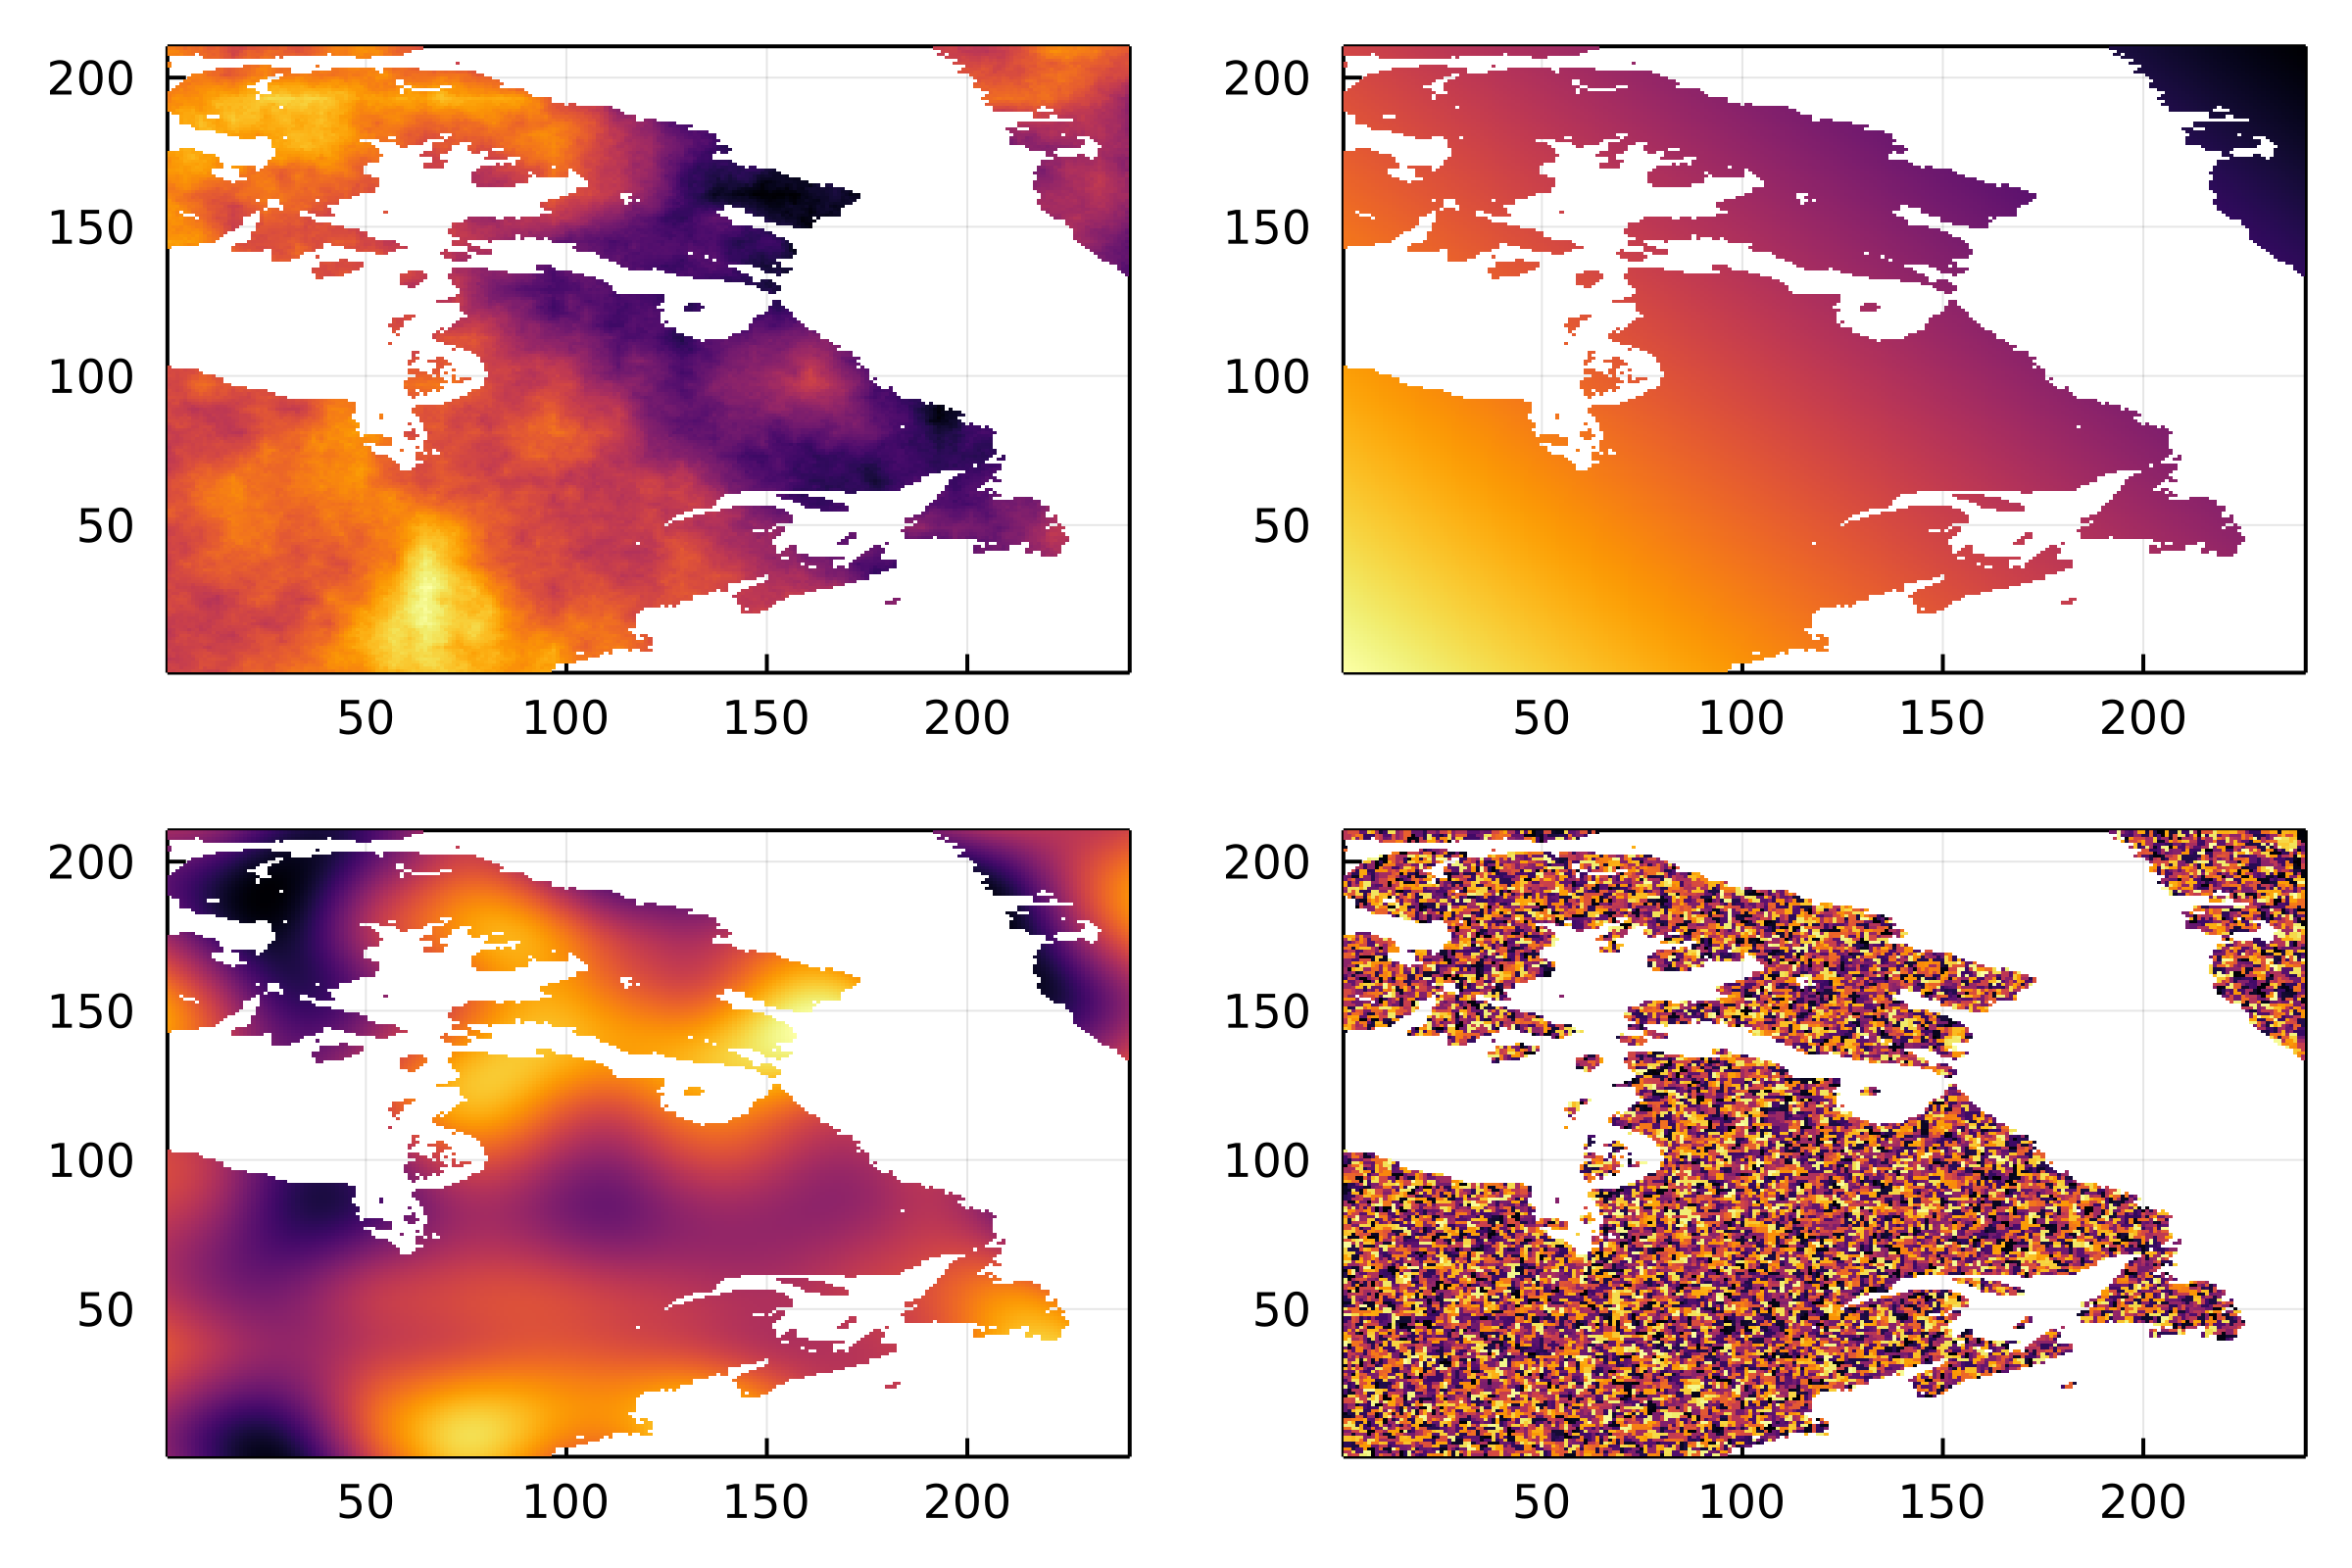
\includegraphics{./figures/interoperable.png}
\caption{todo}
\end{figure}

\hypertarget{benchmark-comparison-to-nlmpy-and-nlmr}{%
\section{\texorpdfstring{Benchmark comparison to \texttt{nlmpy} and
\texttt{NLMR}}{Benchmark comparison to nlmpy and NLMR}}\label{benchmark-comparison-to-nlmpy-and-nlmr}}

It's fast. As the scale and resolution of raster data increases, neutral
models must be able to scale to match those data dimensions. Here we
provide two benchmark tests. First a comparison of the speed variety of
methods from each \texttt{NeutralLandscapes.jl}, \texttt{NLMR}, and
\texttt{nlmpy}. Second we compare these performance of each of these
software packages as rasters become larger. We show that \texttt{Julia}
even outperforms the \texttt{NLMR} via C++ implemention of a
particularly slow neutral landscape method (midpoint displacement).

\begin{figure}
\centering
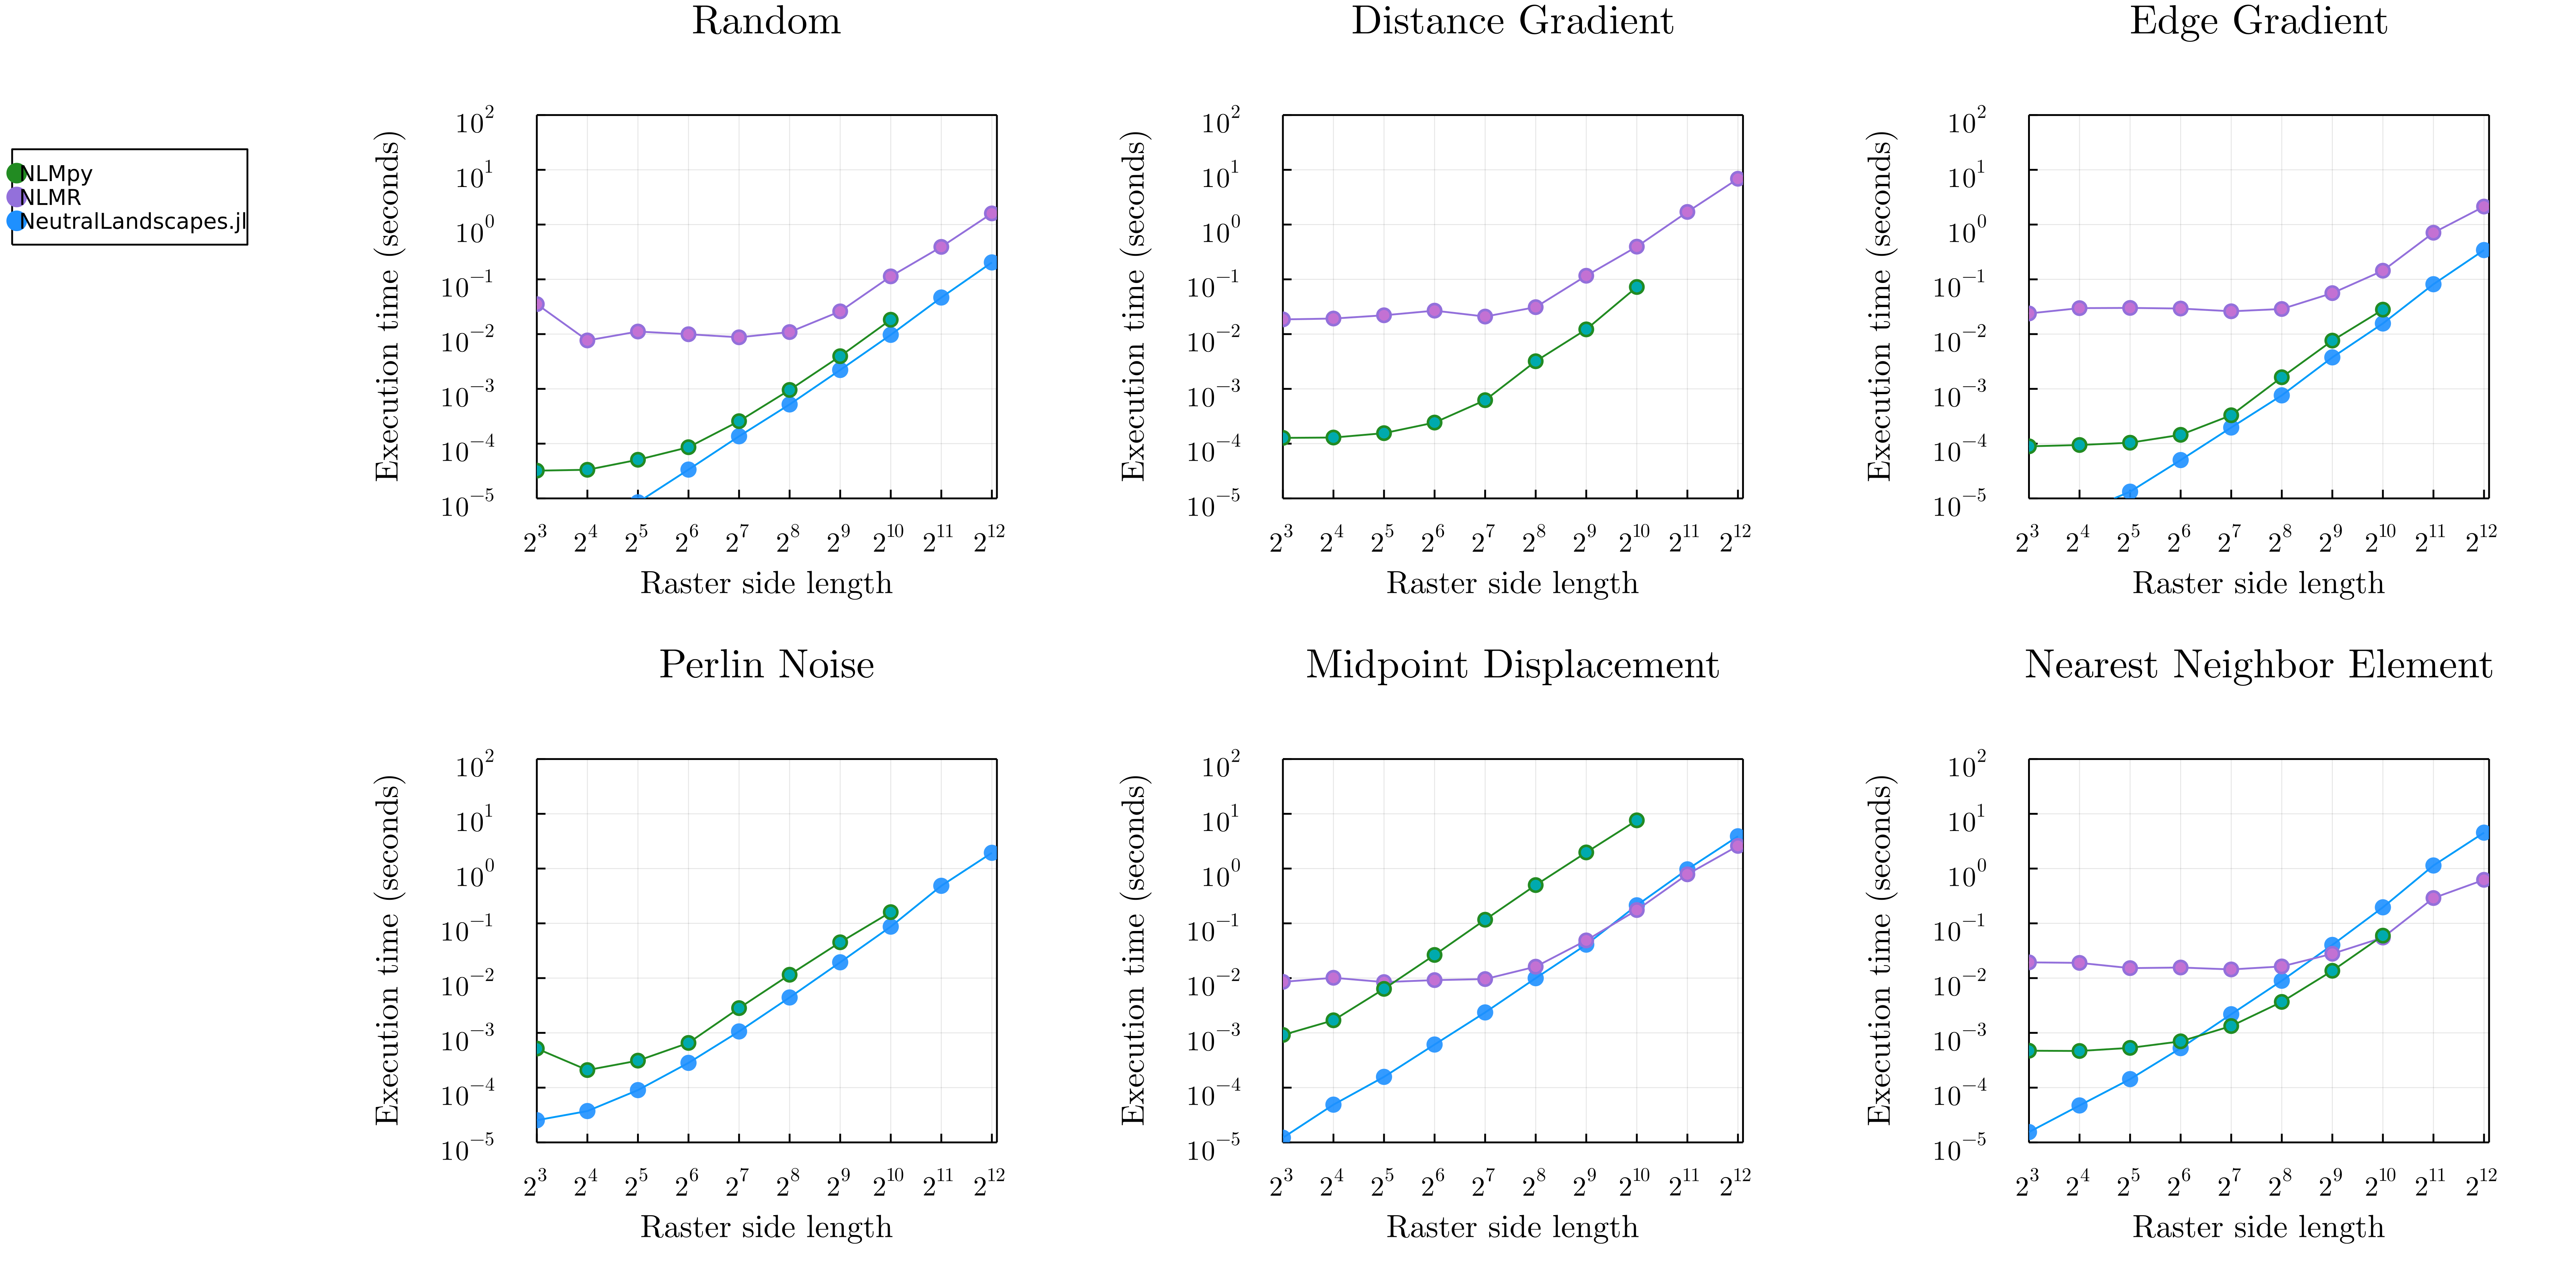
\includegraphics{./figures/benchmark.png}
\caption{todo}
\end{figure}

\hypertarget{generating-dynamic-neutral-landscapes}{%
\section{Generating dynamic neutral
landscapes}\label{generating-dynamic-neutral-landscapes}}

We implement methods for generating change that are temporally
autocorrelated, spatially autocorrelated, or both.

\(M_t = M_{t-1} + f(M(t-1))\)

\hypertarget{models-of-change}{%
\subsection{Models of change}\label{models-of-change}}

\hypertarget{directional}{%
\subsubsection{Directional}\label{directional}}

\hypertarget{temporally-autocorrelation}{%
\subsubsection{Temporally
autocorrelation}\label{temporally-autocorrelation}}

\(r\): rate, \(v\): variability, \(U\) matrix of draws from standard
\(\text{Normal}(0,1)\)

\(f_{T}(M_{ij}) = r + vU_{ij}\)

\hypertarget{spatial-autocorrelation}{%
\subsubsection{Spatial autocorrelation}\label{spatial-autocorrelation}}

\(r\): rate, \(v\): variability, \([Z(\delta)]_{ij}\): the \((i,j)\)
entry of the zscore of the \(\delta\) matrix

\(f_{S}(M_{ij}) = r + v \cdot [Z(\delta)]_{ij}\)

\hypertarget{spatiotemporal-autocorrelation}{%
\subsubsection{Spatiotemporal
autocorrelation}\label{spatiotemporal-autocorrelation}}

\hypertarget{rescaling-to-mimic-real-data}{%
\subsection{Rescaling to mimic real
data}\label{rescaling-to-mimic-real-data}}

\hypertarget{discussion}{%
\section{Discussion}\label{discussion}}

\hypertarget{references}{%
\section{References}\label{references}}

\end{document}
